\documentclass[a4paper, 11pt, titlepage]{article}
\usepackage{fancyhdr}
\usepackage{graphicx}
\usepackage{imakeidx}
\usepackage{makeidx}
\usepackage{mathtools}
\usepackage[spanish]{babel}
\usepackage{eurosym}
\usepackage{hyperref}
\usepackage{amssymb}
\usepackage{listings}
\usepackage{xcolor}

\setcounter{secnumdepth}{5}
\setcounter{tocdepth}{5}

\title{Robustecimiento y securización SSH}
\author{Francisco Javier Balón Aguilar}

\begin{document}

\maketitle
\renewcommand{\contentsname}{Índice}
\tableofcontents
\newpage

\section*{Prólogo}
\newpage

\section{Introducción a SSH}

    SSH --o Secure Shell-- es uno de los protocolos más interesantes de los que se dispone 
    en la administración de sistemas, permitiendo acceder a otros equipos de forma remota; 
    pero sobretodo, de forma segura.
    
    Con SSH creamos un túnel entre cliente y servidor que simula, en la capa de aplicación, 
    la shell o intérprete de comandos del servidor, dotando al administrador de prácticamente 
    toda funcionalidad en el equipo.

    Generalmente se suele equiparar el protocolo SSH con el protocolo Telnet, ya que ambos 
    pretenden una funcionalidad similar. Aun así, existen diferencias notables, esencialmente 
    en la seguridad de las comunicaciones; ya que SSH utiliza técnicas criptográficas para 
    proteger los datos intercambiados entre ambos nodos que conforman la conexión SSH. SSH 
    utiliza un intercambio de claves basado en el protocolo criptográfico de \textit{Diffie-Hellman}, 
    imprescindible en el robustecimiento de la capa de transporte.

    Como vemos, SSH proporciona un sistema, a priori, seguro. Con una configuración con un 
    nivel aceptable de seguridad por defecto. Pero en función de la configuración del 
    servicio puede llevar al sistema a un estado de inseguridad. Por ello, es importante 
    entender el funcionamiento del protocolo, las funcionalidades que presenta y la configuración
    óptima en función de las necesidades del administrador. Este será el núcleo del presente 
    documento.

\section{Visión técnica del protocolo}

    Una vez introducido el protocolo, podemos arremangarnos y entrar en barro. El protocolo 
    SSH trabaja sobre el protocolo TCP/IP. Por ello, en primer lugar se realiza la conexión 
    TCP, realizando el \textit{three-way handshake}\footnote{
        \textit{Three-way handshake} o \textit{triple apretón de manos} es un método 
        utilizado en una red TCP/IP para crear una conexión entre un cliente local y 
        un servidor.

        Es un método de tres pasos en ambas direcciones simultáneamente diseñado para 
        permitir que ambos extremos de comunicación inicien y negocien los parámetros 
        de la conexión de socket TCP antes de que se transmitan datos.

        \[SYN, SYN+ACK, ACK\]
    }. Después de abrir la conexión, cliente y servidor se envían la versión disponible 
    del protocolo\footnote{ \label{versiones}
        Actualmente existen dos versiones del protocolo SSH; la versión 1 y la 2. La primera 
        es actualmente desaconsejable por motivos de seguridad, que son suplidos en la segunda 
        versión.
    }. Después, se utilizará el par de claves, pública y privada, de RSA. El servidor enviará 
    su clave pública de \textit{host} al cliente, de forma que éste pueda cifrar lo que necesite 
    enviar al servidor. El cliente comparará la clave pública de \textit{host} con la que 
    tenga almacenada del servidor en el archivo \textit{known\_host}, si lo hubiera. 

    \begin{figure}[htp]
        \centering
        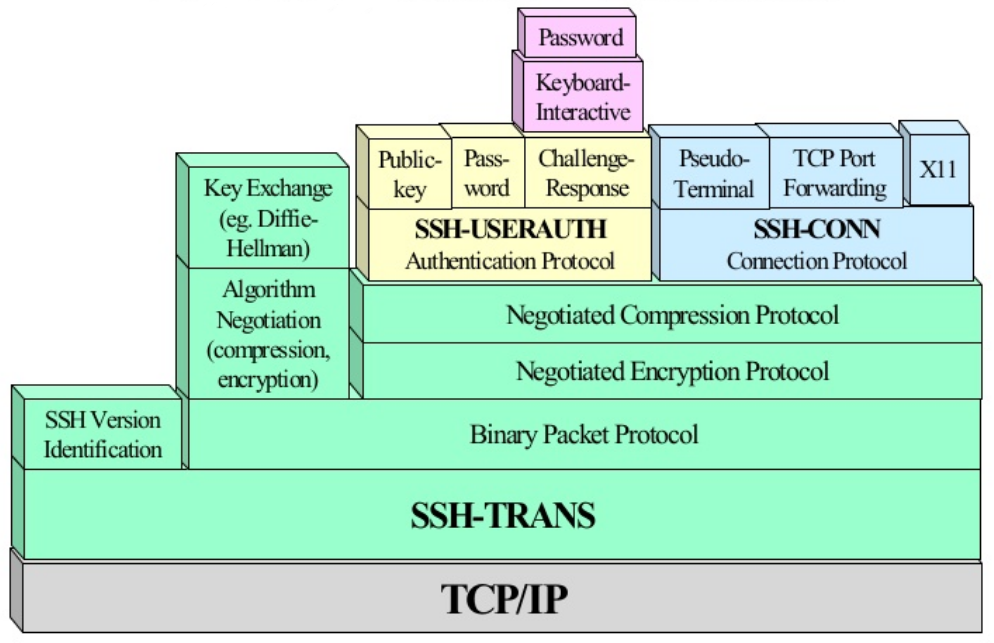
\includegraphics[width=0.8\textwidth]{resources/ssh00.png}
        \caption{Capas del protocolo SSH.}
        \label{ssh00}
    \end{figure}

    Una vez el cliente dispone de la clave pública del \textit{host} del servidor, este 
    generará una clave de sesión aleatoria y seleccionará un algoritmo de cifrado simétrico.
    Con esta clave de sesión, que se generará por defecto cada 3600 segundos, se cifrará el 
    túnel. El cliente enviará un mensaje que contiene la clave de sesión y el algoritmo de 
    cifrado seleccionado, información que viajará cifrada mediante la clave pública de \textit{host},
    al servidor. En este instante, el resto de la comunicación se utilizará el algoritmo de 
    cifrado simétrico y la clave compartida de sesión, dando velocidad a la conexión (en técnicas 
    de clave simétrica el cifrado y descifrado se hace más rápido), pero utilizando siempre 
    primero el protocolo de \textit{Diffie-Hellman} para poder enviar de forma segura 
    la clave compartida de sesión; y supliendo así la principal carencia en seguridad de los algoritmos 
    de criptografía simétrica: el intercambio de claves.

    Una vez tenemos el túnel creado, se llevará a cabo la autenticación del usuario en el 
    servidor, pudiendo utilizar distintos métodos para llevar a cabo tal autenticación.

\section{Instalación de servidor y cliente}

    La instalación tanto del cliente como del servidor es un proceso muy sencillo que no 
    ocupará mucho en la práctica. Debido que estamos utilizando la distribución Arch GNU/Linux, 
    utilizaremos el gestor de paquetes \textit{pacman}, en el que basa la distribución y que, 
    en código, no es más que una pantalla que realiza instalaciones de códigos fuentes \textit{tarballs}
    de forma automatizada. En caso de usar otra distribución, será necesario descargar el paquete 
    \textit{deb} (en aquellas distribuciones basadas en Debian) o \textit{rpm} (en aquellas distribuciones 
    basadas en Red Hat).

    \begin{figure}[htp]
        \centering
        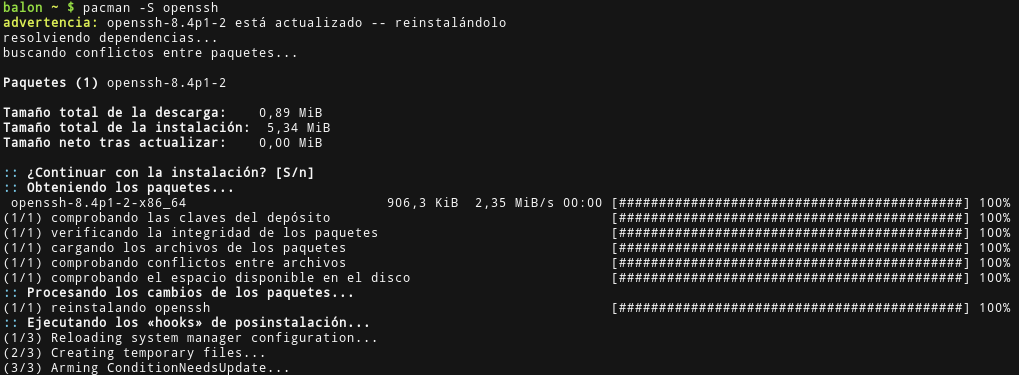
\includegraphics[width=1\textwidth]{resources/ssh01.png}
        \caption{Prueba de instalación de \textit{openssh} usando \textit{pacman}.}
        \label{ssh01}
    \end{figure}

    El paquete donde se encuentra es \textit{openssh}, que nació como alternativa libre a \textit{SSH 
    Communications Security} y que forma parte del proyecto OpenBSD.

\section{Configuración del servicio}

    Podemos clasificar la configuración de SSH en dos grupos: el directorio \textit{/etc/ssh} y el demonio 
    \textit{sshd}. El servidor o demonio cuenta con un fichero de configuración propio (\textit{/etc/ssh/sshd\_config}), 
    mientras que el cliente cuenta con otro en el mismo directorio (\textit{/etc/ssh/ssh\_config}). Es necesario 
    destacar que, en el caso del cliente, si un usuario dispone de un archivo de configuración 
    en su directorio \textit{\$HOME}, será este último preferente y será la configuración que se 
    cargue. Esto permite a una misma máquina tener tantas configuraciones como usuarios en el sistema.
    
    En las siguientes líneas estudiaremos brevemente distintos archivos, al menos los de uso 
    general y los que más nos interesan en la presente práctica; siendo éstos los archivos referentes a 
    la seguridad.

    El primer archivo a tener en cuenta es \textit{moduli}, situado en la ruta \textit{/etc/ssh}. Contiene 
    grupos de \textit{Diffie-Hellman}, los cuales son usados para el intercambio de claves, como 
    ya vimos anteriormente y cuyo procedimiento es imprescindible para la creación de una capa segura 
    de transporte.

    En esta ruta anterior, o bien en la ruta personal de cada usuario (\textit{\$HOME/.ssh/}) encontramos 
    los pares de claves (o una sóla). Estos son los archivos que referencian a la clave privada, 
    y lo que referencian a las claves públicas alojadas (generalmente bajo la extensión \textit{.pub}).

    En la ruta \textit{\$HOME/.ssh/} podemos encontrar además al archivo \textit{Authorized\_keys}, que 
    contiene un listado de claves públicas para la autenticación contra sus servidores, reflejando las 
    claves públicas autorizadas por el usuario\footnote{
        Cuando un cliente se conecta a un servidor, y la autenticación se realiza mediante intercambios 
        de pares de claves, se chequea el valor de la clave pública en el listado de \textit{Authorized\_keys}.
        Si el cliente dispone de la clave privada se autenticará el sistema.
    }. También destaca el archivo \textit{Known\_hosts}, que contiene las claves públicas de hosts de los 
    servidores a los que se ha conectado un cliente. Este fichero es importante para asegurarse de la 
    integridad de la conexión, asegurando que nos conectamos al mismo servidor y no a uno suplantado.

    \subsection{Directivas básicas}

        A continuación especificaremos las directivas básicas para la configuración y robustecimiento 
        del servidor SSH, también el cliente. Estas directivas son informadas en los directorios 
        \textit{sshd\_config} y \textit{ssh\_config}.

        En primer lugar, estas son algunas de las directivas referentes al fichero \textit{sshd\_config}, 
        cuya configuración mejoraría notablemente la seguridad del servidor.

        \begin{itemize}
            \item \textbf{Port}. Esta directiva indica el puerto donde se colocará la escucha del servidor 
            SSH. Por defecto, es el puerto 22. Es interesante de cara a la seguridad no usar el puerto por defecto, 
            de forma que un posible atacante no lo encuentre con tanta facilidad. Se recomienda utilizar puertos en 
            rangos altos, para aumentar el tiempo de búsqueda y esquivar escaneos simples.
            \item \textbf{PermitRootLogin}. Con esta directiva se prohíbe que un usuario se loguee en el servidor
            como \textit{root}, de tal modo que se evita ataques por fuerza bruta al usuario \textit{root}, o 
            bien se haya obtenido anteriormente las claves de acceso a éste; evitando que pueda acceder con 
            los máximos privilegios.
            \item \textbf{MaxAuthTries}. Esta directiva evita que los ataques de fuerza bruta puedan estar probando 
            credenciales indefinidamente, limitando los intentos a un número bajo. Si una vez superado el número de 
            intentos informados el usuario no logra autenticarse correctamente, el sistema abortará la conexión.
            \item \textbf{LoginGraceTime}. Indica el tiempo máximo, en segundos, para introducir las credenciales de 
            autenticación. Es aconsejable utilizar un tiempo bajo, en torno a los 30 segundos (en función claro, de los 
            elementos de seguridad que haya entre cliente y servidor). Evidentemente, no debe ser demasiado bajo 
            ya que podría ocasionar problemas a los usuarios legítimos para acceder.
            \item \textbf{AllowGroups}. De esta forma se le indica al servidor el nombre de los grupos a los que 
            pertenecen los usuarios que tienen permitido el acceso al servidor. En un entorno corporativo, puede ser 
            interesante decidir qué departamentos pueden iniciar sesión o qué grupo de usuarios con privilegios 
            pueden realizr dicha acción.

            \begin{figure}[htp]
                \centering
                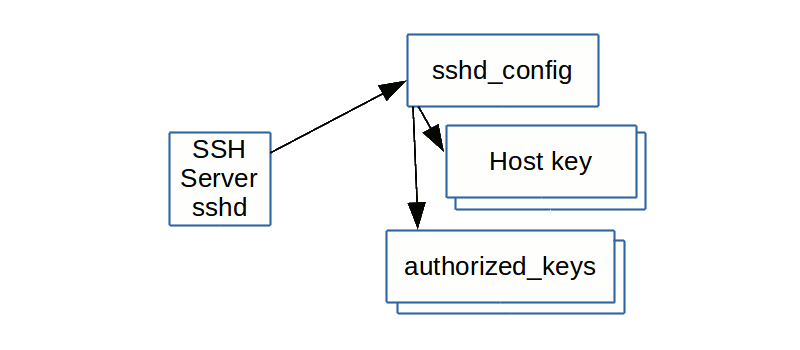
\includegraphics[width=0.8\textwidth]{resources/ssh02.png}
                \caption{Diagrama de ficheros componentes del demonio \textit{sshd}.}
                \label{ssh02}
            \end{figure}        

            Una vez habilitada esta directiva se restringe el acceso a todos los usuarios, a excepción de los que
            pertenezcan a un grupo habilitado.
            \item \textbf{AllowUsers}. Similar a \textit{AllowGroups}, en ésta se indican directamente los usuarios 
            que tienen permitido el acceso. Cabe destacar que se pueden usar metacaracteres, como \$ ó ?, permitiendo 
            la construcción de patrones.
            \item \textbf{Ciphers}. Especifica los cifrados que admitirá el protocolo, por ejemplo 
            \textit{aes128-cbc} ó \textit{blowfish-cbs}.
            \item \textbf{ClientAliveInternal}. Si el servidor no recibe datos del cliente conectado en $x$ tiempo, el 
            servidor enviará un mensaje a través del canal solicitando respesta del cliente.
            \item \textbf{ClientAliveCountMax}. Se especifica el número de mensajes que el servidor puede enviar al cliente 
            solicitando respuesta, antes de cerrar la conexión. 
            \item \textbf{TCPKeepAlive}. Deshabilitar esta directiva permite prevenir ataques de 
            suplantación, ataques de tipo \textit{spoofing}.
            \item \textbf{DenyGroups}. Similar a \textit{AllowGroups} pero con un enfoque inverso, de negación. Los usuarios 
            que pertenezcan los grupos incluidos en la directiva no tendrán permitido el acceso.
            \item \textbf{DenyUsers}. Similar a \textit{AllowUsers} pero con un enfoque inverso, de negación. Los usuarios 
            incluidos en la directiva no tendrán permitido el acceso.
            \item \textbf{LogLevel}. Esta directiva es interesante para depurar y monitorizar lo que ocurre en el servicio.
            Los posibles valores son \textit{QUIET}, \textit{FATAL}, \textit{ERROR}, \textit{INFO}, \textit{VERBOSE} y 
            \textit{DEBUG}. De forma predeterminada se indica \textit{INFO}.
            \item \textbf{HostKey}. Indica en qué ruta se encuentra la clave privada, RSA o DSA, del host.
            \item \textbf{UsePrivilegeSeparation}. Permite la separación de privilegios, es decir, divide los procesos del 
            servidor para prevenir la explotación y la posible escalada de privilegios.
            \item \textbf{Protocol}. Indica la versión del protocolo que se usará. Es importante que se encuentre sólo activada 
            la versión 2 (esto fue adelantado en el apéndice \ref{versiones}), ya que hay versiones en las que esta directiva se 
            especifica como \textit{protocol 2,1}, indicando que si el cliente no dispone de la versión 2 se utilizará la 1. 
            Esto no es nada aconsejable, por lo qeu si el cliente no dispone de la versión 2, es más conveniente denegar la 
            conexión hasta que no actualice su configuración.
            \item \textbf{PubkeyAuthentication}. Permitirá al servidor la autenticación de usuarios mediante el intercambio 
            de clave pública. En entornos críticos es altamente recomendable habilitar este método y deshabilitar otros menos
            seguros (para mayor detalle técnico véase la sección \ref{PubkeyAuthentication}).
            \item \textbf{AuthorizedKeysFile}. Indica, si cambiáramos de directorio, dónde se encuentran almacendas 
            las claves públicas de los usuarios.
            \item \textbf{PasswordAuthentication}. Si esta directiva se encuentra en valor verdadero \textit{yes}, el servidor 
            permitirá la autenticación de usuarios mediante clave o contraseña. Esto no es recomendable en entornos críticos, en cuyo 
            caso se deberá indicar bajo el valor booleano falso, o \textit{no} en este caso (para mayor detalle técnico véase la sección
            \ref{PasswordAuthentication}).
            \item \textbf{X11Forwarding}. Indica si se permite el reenvío de \textit{X11} a través de la conexión SSH (para mayor 
            detalle técnico véase la sección \ref{X11Forwarding}).
            \item \textbf{ListenAddress}.Indica por cuál interfaz/dirección se deben escuchar las peticiones. Puede que el 
            servidor donde se encuentre el servicio SSH cuente con varias tarjetas de red, y que por seguridad sólo se requiera acceso 
            con la interfaz de red que comunica el servidor con una red interna concreta, por ejemplo.
            \item \textbf{ServerKeyBits}. Indica el tamaño de la clave de sesión. Es altamente recomendable utilizar un tamaño de 
            clave mayor de 786 bits, valor por defecto en muchas versiones del aplicativo. Valores recomendados serían 
            1024 ó 2048 bits.
            \item \textbf{KeyRegenerationInterval}. Indica el tiempo, en segundos, que transcurrirá hasta que se genere una nueva 
            clave de sesión. Por defecto se utiliza un valor de 3600 segundos (1 hora). Este valor por defecto es aceptable en niveles 
            de seguridad, pero si queremos manejar una mayor seguridad podríamos bajarlo más.
            \item \textbf{Banner}. Muestra el texto de advertencia (por ejemplo advirtiendo temas legales sobre un posible 
            acceso no autorizado). El contenido por defecto en caso de no haber la directiva se encuentra en \textit{/etc/issue.net}.
            \item \textbf{PrintLastLog}. Se registra el último inicio de sesión del usuario.
        \end{itemize}

        Una vez estudiadas las directivas principales del servicio o demonio \textit{sshd}, veremos a continuación las del 
        lado del cliente (recordamos que el cliente SSH se configura en \textit{ssh\_config}). Por la propia naturaleza del 
        cliente y como es de esperar, las configuraciones de seguridad son menores; puesto que el núcleo a robustecer es 
        el servidor.

        \begin{itemize}
            \item \textbf{Host}. Actúa como divisor de secciones. De tal forma que, puedan ser configuradas distintas directivas 
            para distintas conexiones con servidores.
            \item \textbf{Port}. Indica el puerto al que se conectará en el servidor.
            \item \textbf{Protocol}. Indica la versión del protocolo a usar por el cliente. Evidentemente, ésta por razones de 
            seguridad debe ser 2.
            \item \textbf{IdentifyFile}. Indica dónde se encuentra almacenada la clave privada.
            \item \textbf{PubkeyAuthentication}. Indica al cliente si se puede autenticar contra el servidor mediante 
            autenticación de clave pública (para mayor detalle técnico véase la sección \ref{PubkeyAuthentication}). 
            \item \textbf{StrictHostKeyChecking}. Define qué realizará el cliente al conectarse con un servidor del cual no 
            se dispone de clave pública de host. En caso booleano verdadero, el cliente aceptará automáticamente la clave recibida; 
            en caso contrario, rechazará la clave del servidor, cerrando la conexión (será necesario añadir manualmente la clave 
            pública para poder conectar). Un tercer valor, \textit{ask}, pide confirmación al usuario en el momento de la 
            conexión.
            \item \textbf{Ciphers}. Lista de algoritmos de cifrado simétrico que puede utilizar el cliente.
            \item \textbf{PasswordAuthentication}. Indica si el cliente puede autenticarse contra el servidor mediante contraseña 
            (para mayor detalle técnico véase la sección \ref{PasswordAuthentication}).
        \end{itemize}

    \subsection{Autenticación básica con contraseña}\label{PasswordAuthentication}

        El método más común y utilizado para autenticación de servicios SSH es el de autenticación con contraseña. Es además 
        el método más sencillo y que menos código e infraestructura requiere; por eso es considerado como la autenticación 
        básica, dando nombre a la presente sección.

        Por razones obvias, existen determinados entornos en los que esta autenticación no debe estar aprobada ni permitida 
        por razones de seguridad, ya que en circunstancias normales y defectuosas, este método permite divesos ataques, en especial 
        ataques de fuerza bruta a usuarios y contraseñas, ataques de diccionario, usuarios con keyloggers...

    \subsection{Autenticación mediante par de claves}\label{PubkeyAuthentication}

        

    \subsection{Proceso de conexión}
\section{Aplicaciones de SSH}
    \subsection{Automatización de contraseñas con \textit{sshpass}}

        La utilidad \textit{sshpass} permite cierta automatización a los administradores a la hora de 
        gestionar conexiones SSH desde otros programas y/o scripts. Esta utilidad sólo funcionará con 
        el modelo de autenticación básica con contraseña (véase sección \ref{PasswordAuthentication}).

        La utilidad sshpass está diseñada para ejecutar SSH utilizando el modo de autenticación de 
        contraseña interactiva de teclado, pero de una manera no interactiva, utilizando acceso TTY 
        directo para garantizar que la contraseña sea emitida por un usuario de teclado interactivo, 
        engañando a SSH haciéndole creer que está obteniendo la contraseña de un usuario interactivo.

        Su modo de uso es tan sencillo como indicar previamente a la comunicación con el servidor SSH 
        la clave de éste tras el comando propio de \textit{sshpass}:

        \begin{lstlisting}[language=bash,basicstyle=\footnotesize]
    $ sshpass -p !4u2tryhack ssh user@host\end{lstlisting}

    \subsection{SCP}
    \subsection{SFTP}
    \subsection{SSHFS}
    \subsection{X11 forwarding}\label{X11Forwarding}
    \subsubsection{Fail2ban}
\section{Tunneling}
    \subsection{Túneles TCP/IP con port forwarding}
\section{SOCKS}

% BIBLIOGRAFÍA Y REFERENCIAS
\newpage
\begin{thebibliography}{X}
    \bibitem{} Hardening de servidores GNU/Linux, Carlos Álvarez Martín \& Pablo González Pérez, Ed. 0xWord
    \bibitem{} sshd\_config - SSH Server Configuration \\ \url{https://ssh.com/ssh/sshd_config/}
    \bibitem{} ssh\_config - SSH Config File \\ \url{https://www.ssh.com/ssh/config/}
    \bibitem{} SSHFS: Mounting a remote file system over SSH \\ \url{https://www.redhat.com/sysadmin/sshfs}
    \bibitem{} SSH password automation in Linux with sshpass \\ \url{https://www.redhat.com/sysadmin/ssh-automation-sshpass}
    \bibitem{} Eight ways to protect SSH access on your system \\ \url{https://www.redhat.com/sysadmin/eight-ways-secure-ssh}
    \bibitem{} Using ssh-keygen and sharing for key-based authentication in Linux \\ \url{https://www.redhat.com/sysadmin/configure-ssh-keygen}
    \bibitem{} Set up SSH access with session recording and containerized bastion servers \\ \url{https://www.redhat.com/sysadmin/secure-session-recording}
    \bibitem{} Setting up containerized SSH servers for session recording with tlog \\ \url{https://www.redhat.com/sysadmin/session-recording-tlog}
\end{thebibliography}

\end{document}